\documentclass{article}

% if you need to pass options to natbib, use, e.g.:
% \PassOptionsToPackage{numbers, compress}{natbib}
% before loading rl_project.

% to compile a camera-ready version, add the [final] option, e.g.:
\usepackage[final]{rl_project}

% to avoid loading the natbib package, add option nonatbib:
% \usepackage[nonatbib]{rl_project}

\usepackage[utf8]{inputenc} % allow utf-8 input
\usepackage[T1]{fontenc}    % use 8-bit T1 fonts
\usepackage{hyperref}       % hyperlinks
\usepackage{url}            % simple URL typesetting
\usepackage{booktabs}       % professional-quality tables
\usepackage{amsfonts}       % blackboard math symbols
\usepackage{nicefrac}       % compact symbols for 1/2, etc.
\usepackage{microtype}      % microtypography
\usepackage{graphicx}

\usepackage{natbib}
\setlength{\bibhang}{0pt}
\newcommand*{\urlprefix}{Available from: }
\newcommand*{\urldateprefix}{Accessed }
\bibliographystyle{bathx}

\title{Social DriveNet: Integrating DDQN with Social Attention for Autonomous Traffic Navigation}


% The \author macro works with any number of authors. There are two
% commands used to separate the names and addresses of multiple
% authors: \And and \AND.
%
% Using \And between authors leaves it to LaTeX to determine where to
% break the lines. Using \AND forces a line break at that point. So,
% if LaTeX puts 3 of 4 authors names on the first line, and the last
% on the second line, try using \AND instead of \And before the third
% author name.

\author{
  Leone Lage Perdigão
  \\
  Department of Computer Science\\
  University of Bath\\
  Bath, BA2 7AY \\
  \texttt{llp31@bath.ac.uk} \\
  %% examples of more authors
  %% \And
  %% Coauthor \\
  %% Affiliation \\
  %% Address \\
  %% \texttt{email} \\
  %% \AND
  %% Coauthor \\
  %% Affiliation \\
  %% Address \\
  %% \texttt{email} \\
  %% \And
  %% Coauthor \\
  %% Affiliation \\
  %% Address \\
  %% \texttt{email} \\
  %% \And
  %% Coauthor \\
  %% Affiliation \\
  %% Address \\
  %% \texttt{email} \\
}

\begin{document}

\maketitle

\section{Problem Definition}

This research project is inspired by and builds upon the paper ''Social Attention for Autonomous Decision-Making in Dense Traffic'' \citep{leurent2019social} with significant modifications aimed at exploring the efficacy of Double Deep Q-Network (DDQN) in complex traffic scenarios. This study aims to validate a possible decision-making enhancement in dense traffic by integrating social attention mechanisms, a novel approach designed to model and predict the behaviors of surrounding drivers in a dynamic and densely populated environment.

As such, the project enfolds both a baseline Deep Q-Network (DQN) model and a DDQN model with Social Attention. These models are trained and evaluated leveraging the `highway-env` simulation environment, a specialised tool for autonomous driving research that provides realistic traffic scenarios and the ability to simulate intricate vehicular interactions \citep{highway-env}.

\subsection{Environment Overview:}
The `highway-env` simulation environment, developed by \citet{highway-env}, offers a versatile setting for testing and developing autonomous driving algorithms. It simulates a multi-lane highway where the autonomous agent (the ego vehicle) must navigate through traffic, avoid collisions, and make strategic driving decisions. The environment supports various traffic densities and complex driving behaviors, making it an ideal platform for studying the effects of social attention mechanisms in reinforcement learning models.

\textbf{States}:
\begin{itemize}
  \item \textbf{Observations}: The state of the environment is captured through observations that include features such as the presence, position (x, y coordinates), velocity (vx, vy components), and orientation (cosine and sine of the heading angle) of nearby vehicles. The observation space is standardized to include a fixed number (e.g., 15) of nearby vehicles to maintain consistent dimensionality across different traffic situations. These observations can be formatted as vectors in kinematics or as matrices in occupancy grids, detailing the spatial distribution of traffic around the ego vehicle.
\end{itemize}

\textbf{Actions}:
\begin{itemize}
  \item \textbf{Continuous Actions}: The ContinuousAction type allows the agent to directly set the low-level controls of the vehicle kinematics, namely the throttle $a$ and steering angle $\delta$.
  \item \textbf{Discrete Actions}: The action space is discrete, encompassing a set of quantized decision options that the learning agent can execute. These actions typically include:
    \[
    a_t \in \{\mathbf{LANE\_LEFT}, \mathbf{IDLE}, \mathbf{LANE\_RIGHT}, \mathbf{FASTER}, \mathbf{SLOWER}\}
    \]
  Here, `LANE\_LEFT' and `LANE\_RIGHT' correspond to lane change maneuvers, `FASTER' and `SLOWER' adjust the vehicle's speed, and `IDLE' maintains the current state without changes.
\end{itemize}

For the purpose of this study, the Discrete Actions where chosen because their nature simplifies the decision-making process and aligns with the common control strategies used in vehicular navigation systems.

\textbf{Transition Dynamics}:
\begin{itemize}
  \item \textbf{Vehicle Dynamics and Road Interactions}: The transition dynamics describe how the state of the environment evolves in response to the actions taken by the autonomous agent. This includes the kinematics of the vehicle, such as changes in speed and direction, as well as interactions with the road infrastructure and other vehicles, which are all influenced by the physical properties of the vehicle and traffic regulations.
\end{itemize}

\textbf{Reward Function}:
\begin{itemize}
  \item \textbf{General Formulation}: The reward function is designed to encourage optimal driving behavior by combining a velocity component and a collision penalty:
    \[
    R(s_t, a_t) = \alpha \left(\frac{v_t - v_{\mathbf{min}}}{v_{\mathbf{max}} - v_{\mathbf{min}}}\right) - \beta \cdot \mathbf{collision}
    \]
  where $v_t$ is the current velocity, $v_{\mathbf{min}}$ and $v_{\mathbf{max}}$ are the minimum and maximum allowable speeds, respectively, and $\alpha$ and $\beta$ are coefficients weighting the importance of speed maintenance and collision avoidance.
  
  \item \textbf{In Goal-Oriented Scenarios}: For tasks such as parking, the reward function might also include a goal proximity term, which measures the agent's effectiveness in navigating towards a specific target:
    \[
    R(s_t, a_t) = -\gamma \|\mathbf{s}_t - \mathbf{s}_{\mathbf{goal}}\|_p - \beta \cdot \mathbf{collision}
    \]
  where $\|\cdot\|_p$ denotes the p-norm distance to the goal state $\mathbf{s}_{\mathbf{goal}}$, and $\gamma$ is a weighting factor. Nonetheless, this reward function variation is not part of the scope of this work.
\end{itemize}

This framework sets up the autonomous system to learn effective driving policies through simulation, optimizing for both efficiency and safety in complex, densely populated traffic scenarios. The use of social attention mechanisms aims to dynamically incorporate the intentions and relative positions of other traffic participants into the decision-making process, enhancing the overall intelligence and responsiveness of the driving system.

\section{Background}

\subsection{Introduction to Reinforcement Learning}
Reinforcement Learning (RL) provides a framework for learning optimal policies in sequential decision-making problems, where an agent learns to achieve goals by interacting with a dynamic environment. This learning process involves observing the state of the environment, selecting actions, and receiving rewards based on the outcomes of these actions \citep{7339478}.

\subsection{Reinforcement Learning in Autonomous Driving}
In the context of autonomous driving, RL can adaptively refine driving strategies by continually processing vehicular dynamics and environmental feedback. The primary goal is to enhance safety, efficiency, and adaptability in complex and unpredictable traffic scenarios \citep{7339478}.

\subsection{Relevant RL Methods and Their Applications}

\subsubsection{Deep Q-Networks (DQN)}
DQN integrates deep neural networks with the Q-learning algorithm, allowing agents to approximate the optimal action-value function in high-dimensional state spaces typical of driving environments. The algorithm updates the Q-values based on the Bellman equation as follows:
\[
Q^{new}(s_t, a_t) \leftarrow Q(s_t, a_t) + \alpha \left[r_t + \gamma \max_{a}Q(s_{t+1}, a) - Q(s_t, a_t)\right]
\]
Despite its success, DQN is prone to overestimations of Q-values due to the max operation in its update rule, which can lead to suboptimal policy learning, particularly in complex driving scenarios where precise action evaluation is critical \citep{DBLP:journals/corr/HasseltGS15}.

\subsubsection{Double Deep Q-Networks (DDQN)}
To address the overestimation issue in DQN, DDQN modifies the Q-value update mechanism by decoupling the action selection from the target Q-value generation:
\[
Q^{new}(s_t, a_t) \leftarrow Q(s_t, a_t) + \alpha \left[r_t + \gamma Q(s_{t+1}, \arg\max_{a}Q(s_{t+1}, a)) - Q(s_t, a_t)\right]
\]
This approach reduces bias in the learning process, enhancing the stability and reliability of the learning outcomes, which is crucial for safety-critical applications like autonomous driving \citep{8500630}.

\subsubsection{Policy Gradient Methods}
Policy gradient methods such as Proximal Policy Optimization (PPO) and Trust Region Policy Optimization (TRPO) optimize the policy directly by estimating the gradient of the expected return. These methods are particularly useful in continuous action spaces, such as steering angle and acceleration control in autonomous vehicles:
\[
\nabla_{\theta} J(\pi_{\theta}) = \mathbb{E}\left[\sum_{t=0}^{T} \nabla_{\theta} \log \pi_{\theta}(a_t|s_t) (R_t - b(s_t))\right]
\]
PPO and TRPO provide mechanisms to maintain exploration while avoiding large updates that could lead to unstable learning, making them well-suited for the adaptive and interactive nature of driving behaviors \citep{7339478}.

\subsection{Integration of Social Attention Mechanisms}
The integration of social attention mechanisms, as explored in the work by Leurent et al. (2019), represents a significant advancement in modeling interactions among multiple agents, such as vehicles in dense traffic. These mechanisms weight the influence of surrounding agents, enhancing the capability of RL models to make context-aware decisions:
\[
\mathrm{Attention}(Q, K, V) = \mathrm{softmax}\left(\frac{QK^T}{\sqrt{d_k}}\right) V
\]
By focusing on relevant vehicles and their behaviors, social attention enables more nuanced and predictive driving strategies, potentially reducing accidents and improving traffic flow efficiency \citep{leurent2019social}.

\subsection{Assessment of Techniques}
While traditional and advanced RL methods offer substantial benefits in autonomous driving, their effectiveness heavily relies on the quality of the simulation environment, the accuracy of the state representation, and the scalability of the algorithms. Continuous research and development efforts are necessary to address these challenges, ensuring that the RL-based systems can operate reliably in real-world traffic conditions.

\section{Method}

\subsection{Experiment}
The experiment began with an exploration of the `highway-env` simulation environment to understand its observation and state spaces Figure~\ref{fig:initial_visual_inspection}. Initial trials involved visual inspections through random actions to gauge the environment's complexity and responsiveness, establishing a baseline understanding essential for structured algorithm application.

\begin{figure}[ht]
  \centering
  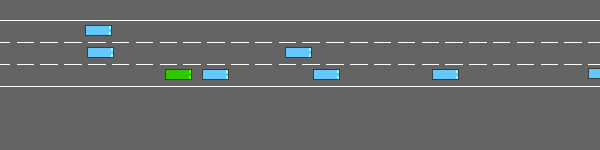
\includegraphics[width=0.5\textwidth]{./figures/highway_simulation_frame7.png}
  \caption{Initial Visual Exploration of Highway-Env}
  \label{fig:initial_visual_inspection}
\end{figure}

The primary intention of the experiment was to test the hypothesis that a Double Deep Q-Network (DDQN) model, enhanced with a social attention mechanism, would significantly outperform the baseline model in navigating dense traffic scenarios.
The experiment's structured approach, from initial exploration to detailed model optimization and evaluation, ensures comprehensive testing and validation of the proposed methods.

\subsection{Baseline DQN Model Architecture}
The baseline DQN model adopts a classical neural network architecture designed to approximate the optimal action-value function \( Q^*(s, a) \), facilitating robust decision-making in dynamic environments \citep{mnih2015humanlevel}:

\begin{itemize}
    \item \textbf{Input Layer:} The architecture takes state inputs corresponding to environmental observations with dimensionality configured for the `highway-env`.
    \item \textbf{Hidden Layers:} Features two hidden layers with 256 neurons each, employing ReLU activation functions \( f(x) = \max(0, x) \) to capture complex patterns in data.
    \item \textbf{Output Layer:} Outputs Q-values for each action in the environment's action space, using linear transformation.
\end{itemize}

This model is optimized using RMSProp, consistent with best practices for training DQNs \citep{mnih2015humanlevel}.

\subsection{Custom DDQN with Social Attention Model Architecture}
The enhanced DDQN model mitigates Q-value overestimations and incorporates a domain-specific social attention mechanism for improved interaction modeling \citep{leurent2019social}:

\textbf{Dual Estimator Configuration:}
\begin{itemize}
    \item \textbf{Policy and Target Networks:} Both networks share identical structures but feature asynchronous updates to reduce biases in value estimation, a method validated in \citep{DBLP:journals/corr/HasseltGS15}.
    \item \textbf{Update Policy:} The target network's parameters are periodically synchronized with the policy network every 50 steps, enhancing prediction stability.
\end{itemize}

\textbf{Social Attention Mechanism:}
The Attention Mechanism pseudocode \citep{DBLP:journals/corr/VaswaniSPUJGKP17}, complementing the mathematical formulation displayed earlier in this report, is defined as:

\begin{verbatim}
Algorithm 1: Social Attention Mechanism
1: procedure Attention(Q, K, V)
2:     d_k <- size of key vectors
3:     scores <- MatMul(Q, Transpose(K)) / sqrt(d_k)
4:     attention_weights <- Softmax(scores)
5:     output <- MatMul(attention_weights, V)
6:     return output
7: end procedure
\end{verbatim}

\textbf{Model Dynamics:}
\begin{itemize}
    \item \textbf{Input Transformation:} Inputs are transformed through linear layers, adapting dimensions suitable for subsequent attention processing.
    \item \textbf{Attention Application:} The attention module processes inputs to focus selectively on significant environmental features, enhancing model responsiveness to dynamic interactions.
    \item \textbf{Sequential Processing:} Features refined through attention are further processed by dense layers, culminating in the output layer that determines action Q-values.
\end{itemize}

The DDQN model with social attention is designed to improve the predictive accuracy and responsiveness of autonomous driving strategies by effectively utilizing dynamic traffic interactions, a concept supported by empirical improvements in traffic navigation tasks \citep{8500630, 9664628}.

\subsection{Hyperparameter Tuning}
Hyperparameter optimization was conducted using the Optuna framework. A range of values for learning rates, batch sizes, discount factors, and network architectures were defined and iteratively tested to maximize the mean reward. The optimal parameters derived from this tuning were subsequently used to retrain the baseline model, thus ensuring optimal baseline performance \citep{optuna_2019}.

\subsection{Model Training and Evaluation}
Following the implementation, both models underwent extensive training in 20.000 episodes. For DDQN, a replay buffer was also used to store and replay past transitions, enhancing the learning from previous experiences. Furthermore, the models were evaluated based on its ability to predict Q-values accurately and make optimal decisions in simulated traffic scenarios \citep{9664628}.

\section{Results}

\subsection{Baseline DQN Model}

The baseline DQN model demonstrates significant learning capabilities through a structured decrease in exploration and consistent improvements in episode length and rewards. The exploration rate's rapid decline indicates an efficient transition from exploring the environment to exploiting learned strategies. Concurrently, increases in episode lengths and rewards reflect the agent's growing proficiency in navigating the environment effectively.

\begin{itemize}
    \item \textbf{Exploration Rate:} Stabilized at a low value (0.05), indicating a shift towards exploitation after initial extensive exploration. Figure \ref{fig:exploration_rate} presents the exploration rate decay over the training period, emphasizing the model's transition from exploration to exploitation.
    \item \textbf{Episode Length:} Showed a progressive increase, suggesting improved decision-making that prolongs episodes. Figure \ref{fig:ep_len_mean} shows the mean episode length over training episodes, providing insight into the agent's ability to maintain effective interaction over time.
    \item \textbf{Episode Rewards:} Exhibited a steady rise, indicative of the agent's enhanced ability to accrue higher rewards. Figure \ref{fig:reward_mean} illustrates the progression of mean rewards per episode, highlighting the agent's increasing efficiency in reward accumulation.
\end{itemize}

These results are depicted in Figures \ref{fig:exploration_rate}, \ref{fig:ep_len_mean}, and \ref{fig:reward_mean}, illustrating the quantitative improvements across these metrics.

\begin{figure}[ht]
  \centering
  \begin{minipage}{0.48\textwidth}
      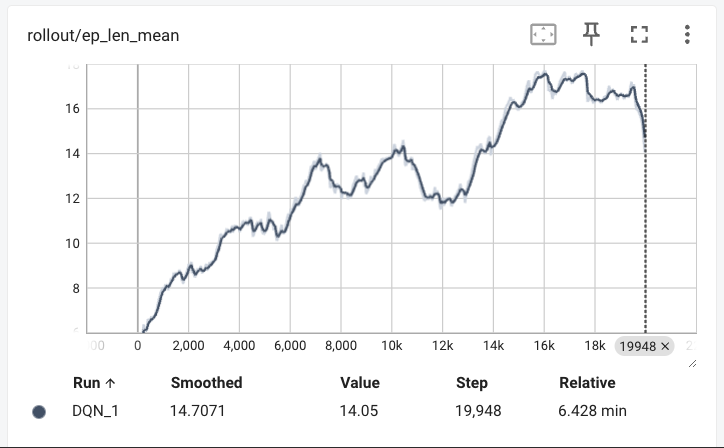
\includegraphics[width=\linewidth]{./figures/dqn_baseline_ep_len_mean.png}
      \caption{Mean episode length}
      \label{fig:ep_len_mean}
  \end{minipage}
  \begin{minipage}{0.48\textwidth}
      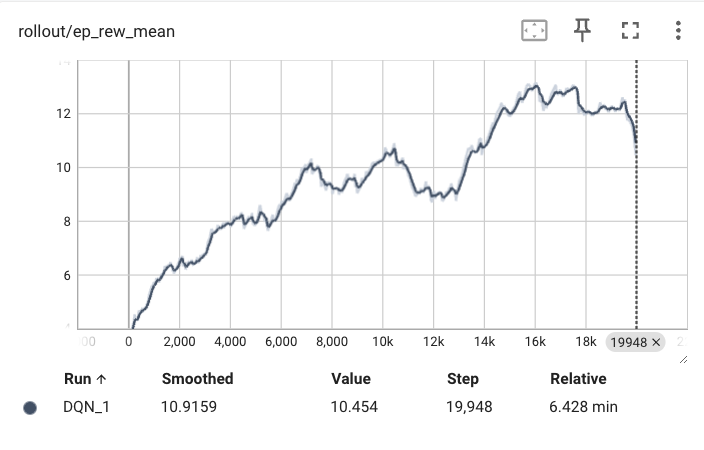
\includegraphics[width=\linewidth]{./figures/dqn_baseline_ep_reward_mean.png}
      \caption{Mean rewards per episode}
      \label{fig:reward_mean}
  \end{minipage}
  \begin{minipage}{0.48\textwidth}
    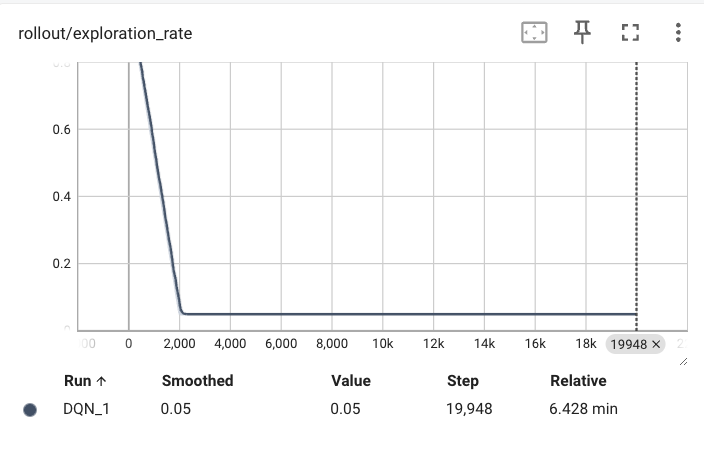
\includegraphics[width=\linewidth]{./figures/ddn_baseline_exploration_rate.png}
    \caption{Exploration rate decay}
    \label{fig:exploration_rate}
  \end{minipage}\hfill
\end{figure}

\subsection{DDQN Model with Social Attention}

The custom DDQN model's training results, analyzed through exponential smoothing and moving average techniques, showcase substantial improvements in reward accumulation, with rewards scaled by a factor of 10 to optimize training. Both smoothing approaches indicate a stable and consistent increase in rewards, highlighting the model's enhanced learning efficiency and its ability to maintain high performance. Exponential smoothing reveals a steady gain in rewards, suggesting robust adaptability, while the moving average confirms a persistent high-level performance toward the end of training. This summary precedes a detailed analysis and comparison with the baseline model, emphasizing the DDQN's superior policy optimization capabilities in complex environments.

Figure \ref{fig:ddqn_exponential} displays the rewards per episode as processed by exponential smoothing, a method that helps in highlighting trends by reducing the influence of outlier rewards or abrupt changes that might not represent the overall learning trajectory.

The graph indicates a gradual and consistent increase in rewards, reaching a stable plateau. This pattern suggests that the DDQN model effectively learns optimal policies over time, with fewer episodes of declining performance, indicating robustness against environmental variations.

Additionally, figure \ref{fig:ddqn_moving_avg} illustrates the rewards per episode using a moving average, which smooths out short-term fluctuations and highlights longer-term trends more clearly.

\begin{figure}[ht]
  \centering
  \begin{minipage}{0.48\textwidth}
      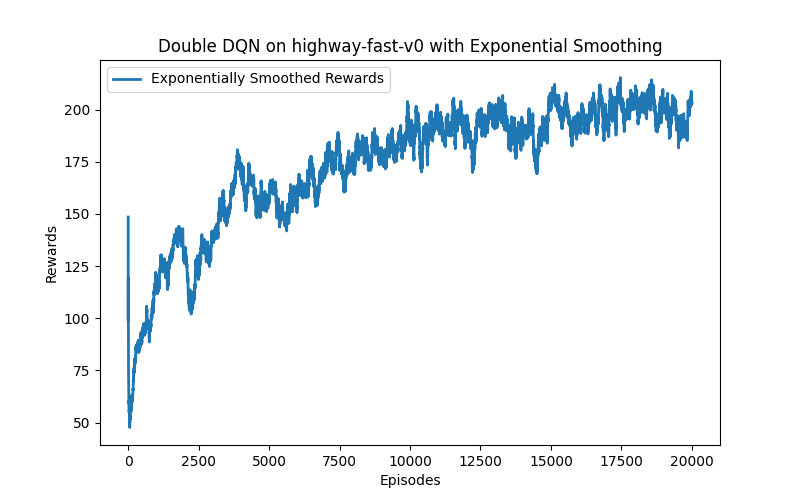
\includegraphics[width=\linewidth]{./figures/ddqn_exponential_smoothing.png}
      \caption{Rewards per episode with exponential smoothing for the DDQN model.}
      \label{fig:ddqn_exponential}
  \end{minipage}
  \begin{minipage}{0.48\textwidth}
      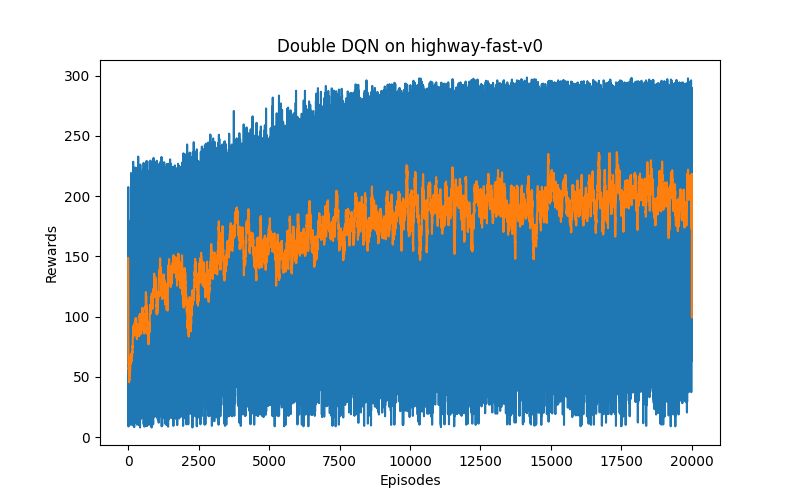
\includegraphics[width=\linewidth]{./figures/ddqn_moving_avg.png}
      \caption{Rewards per episode with a moving average for the DDQN model.}
      \label{fig:ddqn_moving_avg}
  \end{minipage}
\end{figure}

The moving average line (orange) clearly shows a mid-training adjustment where the rewards start to significantly rise, stabilizing at a high level towards the end of the training period. This enhancement indicates the model’s adaptation and refined strategy execution as it encountered different scenarios within the environment.

Overall, both smoothing methods used for the DDQN model—exponential and moving average—provide valuable insights into the learning dynamics. Exponential smoothing gives a closer look at the model's immediate response to changes in episode conditions, while the moving average presents a broader view of the overall performance improvements. The consistency between these two methods in showing upward trends and stabilization in high rewards validates the effectiveness of the DDQN training.


\section{Discussion}

The core objective of this work was to validate the hypothesis of the enhancement of the decision-making capabilities of autonomous vehicles in dense traffic scenarios using advanced reinforcement learning techniques. The baseline DQN model served as the foundation, which we significantly built upon with the DDQN model, integrating a social attention mechanism for improved environmental interaction and decision-making.

The results from the baseline DQN model indicated a competent level of performance with a clear progression in learning, as evidenced by the increase in rewards and episode lengths over training episodes. However, the custom DDQN model exhibited superior performance in several key aspects.

Firtly, concerning \textbf{reward accumulation}, the DDQN model demonstrated a more rapid and stable increase in rewards, a direct indication of its more effective policy optimization. The scaling of rewards by a factor of 10 within the DDQN training regimen likely contributed to this enhanced performance by amplifying the gradients and thus accelerating the learning process.

As for the \textbf{policy stability}, while the baseline DQN showed fluctuations in episode rewards and lengths, the DDQN maintained a more consistent level of high performance. This stability can be attributed to the dual architecture of the DDQN, which reduces the overestimation biases inherent in the standard DQN model \citep{DBLP:journals/corr/HasseltGS15}.

Lastly, regarding \textbf{adaptability}, the integration of a social attention mechanism in the DDQN model allowed for a better adaptation to dynamic traffic scenarios, reflecting a sophisticated understanding of the environment that surpasses the baseline model's capabilities \citep{leurent2019social}.

The findings from this study are consistent with existing literature, which suggests that DDQN models can significantly outperform DQN models in complex decision-making tasks \citep{8500630}. The application of these findings to autonomous driving confirms the potential of advanced reinforcement learning models enhanced by attention mechanisms, not only in achieving higher performance metrics but also in driving practical improvements in autonomous vehicle technology.

\section{Future Work}

This study has showcased promising advancements in reinforcement learning for autonomous driving simulations, yet several challenges persist that require further exploration.

Firstly, while reward scaling has expedited learning, it may mask subtleties in decision-making within complex scenarios \citep{silver2016mastering}. Future research should evaluate the effects of various scaling magnitudes on learning behaviors and performance across diverse reward dynamics. Additionally, the current simulation environment lacks the unpredictability of real-world conditions such as erratic human behavior and environmental changes \citep{dosovitskiy2017carla}. Enhancing simulation fidelity by integrating real-world variables could significantly improve model robustness.

Further investigations should explore richer and more volatile environments by incorporating real-world data, like traffic and accident statistics, to enrich the training context \citep{bojarski2016end}. Moreover, experimenting with different attention mechanisms might enable more precise information prioritization \citep{DBLP:journals/corr/VaswaniSPUJGKP17}, and integrating advanced neural network architectures, such as CNNs for spatial processing and RNNs for temporal data handling, could refine decision-making processes \citep{lecun2015deep}.


\section{Personal Experience}

This project was both challenging and immensely rewarding. Initially planned as a group endeavor with three students, I had to proceed alone due to unresponsive peers. This shift to a solo effort required redefining the project's scope and timelines and necessitated negotiating an extension with our tutor.

Working independently on this demanding project, alongside a full-time job, presented significant stress and workload challenges. The depth of research and the extensive effort needed to implement and fine-tune the reinforcement learning models were at times overwhelming.

Despite these hurdles, the project was very satisfying. Engaging with the field of autonomous vehicles, an area I am passionate about, was particularly rewarding. The process of building, testing, and enhancing the DDQN model, and observing firsthand its improved performance, was gratifying.

This experience underscored the resilience and adaptability required in academia. It drove me to develop new skills, enhancing my capability to work independently and manage unexpected challenges effectively.

\small
\bibliography{references}

\normalsize
\newpage
\section*{Appendices}
\section*{Appendix A: Hyperparameter Selection}

The selection and optimization of hyperparameters were critical to the performance of both the baseline DQN and the custom DDQN models in this project. These parameters were initially chosen based on established practices within the literature and subsequently fine-tuned to optimize each model's learning efficacy and performance in the simulated autonomous driving environment.

\subsection*{Initial Hyperparameter Setup}
The initial hyperparameters for both models were selected based on conventional values recommended in seminal reinforcement learning studies and adjusted through preliminary experimental runs to suit our specific simulation settings.

\subsection*{Automated Hyperparameter Optimization}
To systematically determine the most effective hyperparameters, we employed the Optuna framework, which uses Bayesian optimization to explore the parameter space efficiently. This approach was instrumental in refining the hyperparameters for both models, with the objective to maximize the cumulative rewards obtained per episode.

\subsection*{Final Hyperparameters for DDQN Model}
The optimization process identified the following set of hyperparameters as optimal for the DDQN model:

\begin{itemize}
    \item \textbf{Learning Rate:} \(0.002265898105933512\), which provided a balance between fast convergence and stability in updates.
    \item \textbf{Discount Factor (\(\gamma\)):} \(0.7093581079384662\), reflecting a preference for rewards in the near to medium term, which suited the dynamic conditions of the driving simulation.
    \item \textbf{Exploration Rate (\(\epsilon\)):} Initially set at \(0.8\) and decayed over time, ensuring a robust exploration of the action space early in training.
    \item \textbf{Batch Size:} \(128\), enabling the model to learn from a broader range of experiences in each update, enhancing the generalization of the learned policies.
    \item \textbf{Target Update Frequency:} Every \(100\) steps, providing a good balance between stability and responsiveness in updating the target network.
    \item \textbf{Hidden Dimensions:} Layers with \(256, 256\) neurons, ensuring sufficient complexity to model the decision-making process effectively.
\end{itemize}

A similar strategy was employed for tuning the baseline DQN model, using Optuna to explore various configurations. Although the specific optimal parameters varied slightly due to differences in model architecture, the approach fundamentally remained consistent between the two models.

Future work could continue to refine these parameters and explore additional adjustments to further improve the models' effectiveness in increasingly complex driving scenarios.

\end{document}
